\documentclass[border=10pt]{standalone}
\usepackage{pgfplots}
\usepgfplotslibrary{units}
\pgfplotsset{compat=1.18, trig format plots=rad}
\begin{document}
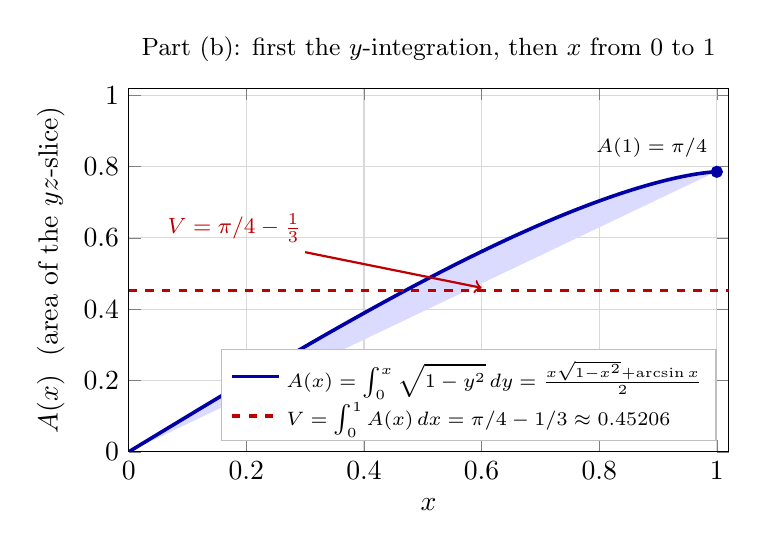
\begin{tikzpicture}
\begin{axis}[
    width=9.2cm, height=6.2cm,
    xmin=0, xmax=1.02, ymin=0, ymax=1.02,
    xlabel=$x$, ylabel={$A(x)$ \ (area of the $y z$-slice)},
    title={Part (b): first the $y$-integration, then $x$ from 0 to 1},
    title style={font=\small},
    grid=major, grid style={black!15},
    legend style={at={(0.98,0.03)}, anchor=south east, font=\scriptsize,
                  fill=white, draw=black!25, cells={anchor=west}}]
    \addplot[blue!65!black, line width=1.3pt, fill=blue!14, domain=0:1, samples=120]
        {0.5*(x*sqrt(1-x^2) + asin(x))};
    \addlegendentry{$A(x)=\int_{0}^{x}\sqrt{1-y^{2}}\,dy
        =\frac{x\sqrt{1-x^{2}}+\arcsin x}{2}$}
    \addplot[red!75!black, dashed, line width=1.2pt, domain=0:1.02, samples=2]
        ({x},{0.45206483});
    \addlegendentry{$V=\int_{0}^{1}A(x)\,dx=\pi/4-1/3\approx 0.45206$}
    \addplot[only marks, mark=*, mark size=2pt, blue!65!black] coordinates {(1,0.78539816)};
    \node[font=\scriptsize, anchor=south east] at (axis cs:1,0.80) {$A(1)=\pi/4$};
    \draw[->, red!75!black, line width=0.8pt] (axis cs:0.30,0.56) -- (axis cs:0.60,0.460);
    \node[font=\footnotesize, text=red!75!black, anchor=south east] at (axis cs:0.31,0.56)
        {$V=\pi/4-\frac{1}{3}$};
\end{axis}
\end{tikzpicture}
\end{document}
